\documentclass[czech,master]{diploma}
\usepackage[autostyle=true,czech=quotes]{csquotes}
\usepackage[backend=biber, style=iso-numeric, alldates=iso]{biblatex}
\usepackage{dcolumn}
\usepackage{subfig}
\usepackage{hyperref}
\usepackage{xurl}
\usepackage{tikz}
\usepackage[cpp]{diplomalst}

\ThesisAuthor{Bc. Filip Peterek}
\ThesisSupervisor{prof. RNDr. Marie Duží, CSc.}
\CzechThesisTitle{Implementace jazyka TIL-Script}
\EnglishThesisTitle{Implementation of the TIL-Script Language}
\SubmissionYear{2023}

\ThesisAssignmentFileName{spec.pdf}

\Acknowledgement{TODO: Doplnit poděkování, až bude práce hotová}

\CzechAbstract{
    Cílem práce je implementovat programovací jazyk TILScript. Jazyk TILScript slouží jako
    výpočetní varianta logického kalkulu TIL, jenž umožňuje jednoduchý strojový zápis konstrukcí
    Transparentní intenzionální logiky, ale také jejich následné provedení. Práce dále řeší
    praktické problémy s interpretací TILScriptu, a to například definice pojmenovaných funkcí,
    interakce s databází, apod. Dále se práce snaží navrhnout nadmnožinu jazyka TILSkript, která
    umožní konstrukce TILu nejen provádět, ale také analyzovat, vytvářet je, a pracovat s nimi.
}

\CzechKeywords{
    Transparentní intenzionální logika, TILScript, překladač
}

\EnglishAbstract{
    The goal of the thesis is the definition and implementation of the TILScript language.
    TILScript is a scripting language which serves the purpose of a computational variant of
    Transparent intensional logic, a logical calculus based on typed lambda calculi. TILScript
    allows for not just representation, but also execution of TIL constructions. This work also
    deals with practical problems of TILScript implementation, such as definitions of named
    functions, interaction with databases, and so on. Furthermore, this thesis attempts to define
    a superset of the TILScript language, which allows for not just the execution of constructions,
    but also for their creation and analysis.
}

\EnglishKeywords{
    Transparent intensional logic, TILScript, interpreter
}

\AddAcronym{TIL}{Transparentní intenzionální logika}
\AddAcronym{JVM}{Java Virtual Machine}

\addbibresource{biblatex-examples.bib}
\addbibresource{coffee.bib}

% Novy druh tabulkoveho sloupce, ve kterem jsou cisla zarovnana podle desetinne carky
\newcolumntype{d}[1]{D{,}{,}{#1}}


% Zacatek dokumentu
\begin{document}

\MakeTitlePages

% TODO
% Jsou v praci obrazky? Pokud ano vysazime jejich seznam a odstrankujeme.
% Pokud ne smazeme nasledujici dve makra.
\listoffigures
\clearpage

% TODO
% Jsou v praci tabulky? Pokud ano vysazime jejich seznam a odstrankujeme.
% Pokud ne smazeme nasledujici dve makra.
\listoftables
\clearpage

% A nasleduje text zaverecne prace.
% \chapter{Úvod}
\label{sec:Introduction}



\endinput

\chapter{Transparentní intenzionální logika}
\label{sec:TILIntroduction}

% TODO: Citace
Transparentní intenzionální logika (TIL) je logický systém založený na typovaném lambda kalkulu.
TIL je využíván k logické analýze přirozeného jazyka. Oproti tradičnímu lambda kalkulu, jenž
se využívá jako komputační model, tedy jako pouhý prostředek k dosažení konkrétní hodnoty --
výsledku, v Transparentní intenzionální logice hraje konstrukce kalkulu často důležitější roli,
než hodnota, kterou by konstrukce po provedení zkonstruovala.

Jako příklad využití lambda kalkulu jako výpočetní model lze uvést např. funkcionální programovací
jazyk Haskell. Interně je Haskell kompilován do lambda kalkulu (přesněji do jeho supersetu
obsahujícího např. čísla nebo logické hodnoty, která jinak v lambda kalkulu musíme kódovat pomocí
Churchova kódování -- K-kombinátorů, apod.). Ultimátně v Haskellu ovšem lambda kalkul slouží pouze
k získání konkrétního výsledku. Nadefinujeme vztah mezi vstupem a výstupem, a program napsaný
v Haskellu nám vstup transformuje. Pokud zanedbáme efektivitu programu, nezajímá nás, jakým
způsobem program spočítal výsledek, dokud jej spočítal správně.

Naopak Transparentní intenzionální logika je hyperintenzionálním kalkulem, který nám umožňuje
vytvářet konstrukce vypovídající o jiných konstrukcích. TIL vychází z myšlenky, že výraz
přirozeného jazyka sice označuje denotát -- konkrétní objekt (např. individuum, číslo, konstrukci),
významem výrazu ovšem není samotný denotát, který ani nemusí nutně existovat. Význam výrazu je
abstraktní procedura a lze jej zachytit konstrukcí. Daná konstrukce poté při provedení zkonstruuje
denotát výrazu. Jako příklad lze uvést například výraz ``francouzský král.'' V době psaní této práce
Francie krále nemá. Denotátem výrazu je tak neobsazená individuová role -- výraz tedy neoznačuje
žádné individuum. Přesto výrazu ``francouzský král'' rozumíme, výraz má svůj význam, jen v současné době neuvádí žádnou osobu.
A budeme-li chtít o významu výrazu ``francouzský král'' něco vypovědět, například že francouzský král
je monarchou v čele Francie, daný monarcha nemusí existovat. Dále lze uvést například rozdíl mezi
výrazy ``logaritmus 1024 o základě 2'' a ``5 + 5''. Denotátem obou výrazů je 10. Zadáme-li do
interpreteru Haskellu výrazy

\lstset{language=Haskell}
\lstinline{logBase 2 1024} a \lstinline{5 + 5}, získáme v obou případech stejný výsledek.
V přirozeném jazyce ovšem chápeme značný rozdíl mezi oběma výrazy, ačkoliv mají stejný denotát.
``Logaritmus 1024 o základě 2'' vyjadřuje číslo, kterým musíme umocnit dvojku, abychom získali 1024.
Výraz ``5 + 5'' očividně vyjadřuje úplně jinou matematickou operaci a jeho výsledek spočítáme jiným
postupem.

\begin{figure}
    \centering
    \begin{tikzpicture}
        \node[draw, fit={(0, 0) (2, 1)},              xshift=3cm, inner sep=0pt, label=center:Výraz] (A) {};
        \node[draw, fit={(0, 0) (2, 1)}, yshift=-5cm,             inner sep=0pt, label=center:Konstrukce] (B) {};
        \node[draw, fit={(0, 0) (2, 1)}, yshift=-5cm, xshift=6cm, inner sep=0pt, label=center:Denotát] (C) {};

        \path (A) -- node[sloped] (ab) {vyjadřuje}  (B);
        \path (A) -- node[sloped] (ac) {označuje}   (C);
        \path (B) -- node[sloped] (bc) {konstruuje} (C);

        \draw [-latex]          (A)--(ab)--(B);
        \draw [-latex] [dashed] (A)--(ac)--(C);
        \draw [-latex]          (B)--(bc)--(C);
    \end{tikzpicture}
    \caption{Schéma procedurální sémantiky TIL}\label{fig:til-semantics}
\end{figure}

Denotátem výrazu může být nejen objekt z báze, ale i konstrukce nebo funkce.

Jak již bylo zmíněno, Transparentní intenzionální logika vychází z typovaného lambda kalkulu, proto
také každý objekt musí mít svůj typ. Pro správné pochopení TILu, a tedy i této práce, je tak nutné 
znát typovou hierarchii TIL.

\section{Objektová báze}

Objektová báze je kolekce vzájemně disjunktních neprázdných množin, které dohromady vymezují
nulární funkce, se kterými budeme pracovat. Bázi volíme dle potřeb konkrétní aplikace a univerza
diskurzu. Například používáme-li TIL k logické analýze matematických vět, jako bázi lze zvolit
například množinu celých čísel, množinu reálných čísel, a množinu pravdivostních hodnot. Musíme
však vzít v potaz, že tato báze neobsahuje čísla komplexní.

Patří-li objekt $x$ do množiny $\alpha$ z báze, říkáme, že se jedná o objekt typu $\alpha$.
K explicitnímu uvedení typu objektu \textit{x} využíváme zápis $x/\alpha$. Množinám tvořícím bázi
lze přirozeně říkat typy.

Pro analýzu přirozeného jazyka se většinou volí objektová báze skládající se z typů {$o$, $\iota$,
$\tau$, $\omega$}. Tyto typy jsou podrobněji popsány v tabulce \peteref{tab:default-base}.

\begin{table}
    \caption{Výchozí báze pro analýzu přirozeného jazyka}\label{tab:default-base}
    \centering

    \begin{tabular} { | l l | }
        \hline
        Typ      & Popis typu \\
        \hline
        $o$      & Množina pravdivostních hodnot \\
        $\iota$  & Množina individuí (univerzum diskurzu) \\
        $\tau$   & Množina časových okamžiků/reálných čísel \\
        $\omega$ & Množina logicky možných světů \\
        \hline
    \end{tabular}
\end{table}

\section{Funkce}\label{fn-arity}

V některých logických systémech, například v predikátové logice, se jako základní molekulární typ
využívají relace. Funkce je poté speciální typ relace, která je zprava jednoznačná. V TIL je však
základním molekulárním typem funkce. Chceme-li v TIL vyjádřit $n$-ární relaci nad množinou
$\alpha_1 \times ... \times \alpha_n$, lze tak samozřejmě udělat definicí $n$-ární funkce
z $\alpha_1 \times ... \times \alpha_n$ do $o$, která každému prvku
z $\alpha_1 \times ... \times \alpha_n$ přiřadí pravdivostní hodnotu na základě toho, zda prvek
do relace patří, nebo ne.

% TODO: https://www.phil.muni.cz/~raclavsky/texty/partiality_til.pdf
Narozdíl od tradičního lambda kalkulu je Transparentní intenzionální logika kalkulem parciálních
funkcí. Z parciality funkcí poté vyplývá další vlastnost TIL -- arita funkcí není shora omezená.
V lambda kalkulech totálních funkcí lze využít Sch{\"o}nfinkelovu redukci k redukci funkcí
$n$-árních na unární za využití skládání funkcí. Tato redukce však není ekvivalentní, pracujeme-li
s funkcemi parciálními.

\subsection{Intenze a extenze}

V TIL dále rozlišujeme funkce na tzv. \textit{intenze} a \textit{extenze}. Intenze jsou funkce
z možných světů. Extenze jsou funkce, jejichž doménou množina možných světů není, a tudíž jejich
funkční hodnota nezávisí na stavu světa.

Intenze jsou obecně funkce typu $(\alpha\omega)$ pro libovolný typ $\alpha$. Nejčastěji se však
jedná o funkce typu $((\alpha\tau)\omega)$, tedy funkce zobrazující možné světy do chronologií
objektů typu $\alpha$.

\section{Konstrukce TIL}

Konstrukce v Transparentní intenzionální logice jsou abstraktní procedury. Tyto procedury jsou
strukturované -- nejedná se o množiny, mají pevně danou strukturu, a na uspořádání případných
podprocedur záleží. Tyto konstrukce lze podle definovaných pravidel provést. Provedením konstrukce
získáme výstup, případně nezískáme nic. Konstrukce, které nekonstruují žádný výstup, nazýváme
\textit{nevlastní} (anglicky \textit{improper}). V TIL pracujeme s šesti druhy konstrukcí.

Jak již bylo zmíněno, konstrukce můžou v TIL operovat nejen nad objekty, které nejsou konstrukcemi,
tedy nad objekty z báze a funkcemi, ale také nad jinými konstrukcemi. Konstrukce však může operovat
pouze nad konstrukcemi nižšího řádu, než je konstrukce samotná, viz \peteref{type-order}. Každou
podkonstrukci, kterou musíme provést při provedení konstrukce, nazýváme \textit{konstituentem}.
V TIL existuje šest různých druhů konstrukcí. Dvě atomické -- mají pouze jeden konstituent, a to
sebe samotné, a čtyři molekulární. Atomickými konstrukcemi jsou \textit{Trivializace} a
\textit{proměnné}. Mezi molekulární konstrukce poté řadíme \textit{Kompozice}, \textit{Uzávěry},
\textit{Provedení} a \textit{Dvojí Provedení}.

\textit{Proměnné} jsou konstrukce, které na základě valuace \textit{v} \textit{v}-konstruují
objekty. Skutečnost, že proměnná $x$ \textit{v}-konstruuje hodnotu typu $\alpha$ značíme
$x \rightarrow_v \alpha$.

\lstset{language=Lisp}
\textit{Trivializace} pro libovolný objekt \textit{X} konstruuje samotný objekt \textit{X}.
Konstrukce je v Transparentní intenzionální logice potřebná, neboť výchozím módem pro konstrukce
je provedení. Samotná konstrukce \textit{X} by tak byla automaticky provedena, a místo konstrukce
\textit{X} bychom dostali pouze její denotát. Pokud bychom chtěli zkonstruovat konstrukci
\textit{X}, musíme ji trivializovat. Tím se provede pouze konstrukce Trivializace. A protože
Trivializace nemá jiný konstituent, než sebe samotnou, konstrukce \textit{X} se tak neprovede.
V literatuře se Trivializace \textit{X} tradičně značí ${}^0X$. Alternativně se používá také zápis
$'X$. Tento zápis je poté využit i v jazyce TIL-Script. Trivializaci lze považovat za ekvivalent
funkce \lstinline{QUOTE} z jazyka Lisp. Trivializace taktéž bývá využívána ke konstruování hodnot,
které nelze provést (objekty z báze, funkce) a tudíž je nelze zmínit netrivializované.
\footnote{
    V jazyce Lisp čísla konstruují sebe samotné, tedy provedením čísla získáme zpět prováděné
    číslo. \lstinline{1} a \lstinline{'1} jsou tedy v Lispu ekvivalentní výrazy. V TIL však není
    možné, aby objekt konstruoval sám sebe, viz rozvětvená hierarchie typů \peteref{type-order}.
}

\textit{Kompozice} je procedura aplikace funkce na argumenty. Kompozice $[X Y_1...Y_m]$ značí
aplikaci funkce konstruované konstrukcí $X$ na argumenty zkonstruované konstrukcemi $Y_1,...,Y_m$.
Pokud konstrukce $X$ $v$-konstruuje funkci $f$, všechny podkonstrukce $Y_1,...,Y_m$ $v$-konstruují
hodnotu, a je-li funkce $f$ na daných argumentech definovaná, kompozice $v$-konstruuje funkční
hodnotu na těchto argumentech. V opačném případě je kompozice $v$-nevlastní.

\textit{Uzávěr} $\lambda x_1...x_m Y$ je konstrukce $v$-konstruující funkci. $x_1,...x_m$ musí
být navzájem různé proměnné, $Y$ musí být konstrukcí. Konstruce uzávěru je velmi podobná abstrakci
v lambda kalkulu. Narozdíl od lambda kalkulu však v TILu může uzávěr konstruovat funkce s aritou
vyšší než jedna. Uzávěr nemůže být nikdy nevlastní, může však konstruovat tzv.
\textit{degenerovanou funkci}, tedy funkci, která je nedefinovaná na celém definičním oboru.

\textit{Provedení} ${}^1X$ je konstrukce $v$-konstruující objekt konstruovaný konstrukcí $X$.
Pokud je konstrukce $X$ $v$-nevlastní, je provedení ${}^1X$ také $v$-nevlastní. Jelikož je však
provedení výchozím módem pro objekty, většinou se neuvádí. Provést lze pouze konstrukce. Objekty
z báze (tedy čísla, individua, apod...) či funkce nelze provést, jejich provedení nekonstruuje nic.
Proto je potřeba tyto objekty vždy trivializovat.

\textit{Dvojí provedení} ${}^2X$ je poslední z výčtu konstrukcí. Je-li $X$ konstrukcí
$v$-konstruující konstrukci $Y$, a $v$-konstruuje-li konstrukce $Y$ objekt $Z$, pak ${}^2X$
$v$-konstruuje $Z$. V opačném případě je dvojí provedení ${}^2X$ $v$-nevlastní.

Jiné konstrukce v Transparentní intenzionální logice neexistují.

\subsection{Princip kompozicionality} 

Princip kompozicionality je důležitým rysem Transparentní intenzionální logiky. Z principu
kompozicionality vyplývá, že je-li libovolný konstituent konstrukce $X$ $v$-nevlastní a pro danou
valuaci $v$ nekonstruuje žádnou hodnotu, pak je $v$-nevlastní i konstrukce $X$.

\section{Typy 1. řádu}\label{fst-order}

% TODO: Doplnit citaci
Definice je skoro slovo od slova převzata z knihy
\textit{TIL jako procedurální logika -- Průvodce zvídavého čtenáře Transparentní intensionální
logikou}. Tato sekce slouží jako krátké vysvětlení základů Transparentní intenzionální logiky
se čtenář může obrátit například na tuto knihu.

Nechť \textit{B} je báze. Pak:

\begin{enumerate}[i)]
    \item Každá množina z báze \textit{B} je atomický typ řádu 1 nad \textit{B}.
    \item Nechť $\alpha, \beta_1, ...,\beta_m (m > 0)$ jsou typy řádu 1 nad \textit{B}. Pak soubor
        všech \textit{m}-árních parciálních funkcí $(\alpha\beta_1...\beta_m)$, tedy zobrazení z 
        $\beta_1 \times ... \times \beta_m$ do $\alpha$, je molekulární typ řádu 1 nad \textit{B}.
    \item Nic jiného není typem řádu 1 nad bází \textit{B}.
\end{enumerate}

\section{Rozvětvěná hierarchie typů}\label{type-order}

%TODO: Doplnit citaci
Definice je opět skoro slovo od slova převzata z Průvodce.

Nechť \textit{B} je báze. Pak:

\subsection{$T_1$ (typy řádu 1)}
Viz sekce \peteref{fst-order}.

\subsection{$C_n$ (konstrukce řádu n)}

\begin{enumerate}[i)]
    \item Nechť $x$ je proměnná $v$-konstruující objekt typu řádu $n$. Pak $x$ je
        \textit{kontrukce řádu n nad B}.
    \item Nechť $X$ je prvek typu řádu $n$. Pak trivializace ${}^0X$, provedení ${}^1X$ a dvojí
        provedení ${}^2X$ jsou \textit{konstrukcemi řádu n nad B}.
    \item Nechť $X, Y_1, ... Y_m$ jsou konstrukce řádu $n$ nad \textit{B}. Pak kompozice 
        $[X Y_1...Y_m]$ je \textit{konstrukce řádu n nad B}.
    \item Nechť $x_1,...,x_m$ jsou vzájemně různé proměnné a $X$ je konstrukce řádu $n$
        nad \textit{B}. Pak uzávěr $[\lambda x_1 ... x_m X]$ je \textit{konstrukce řádu n nad B}.
    \item Nic jiného není konstrukcí řádu $n$ nad bází \textit{B} než dle i)-v).
\end{enumerate}

\subsection{$T_{n+1}$ (typy řádu n+1)}

Nechť $*_n$ je kolekce všech konstrukcí řádu $n$ nad $B$.

\begin{enumerate}[i)]
    \item $*_n$ a každý typ řádu $n$ jsou \textit{typy řádu n+1 nad B}.
    \item Jsou-li $\alpha, \beta_1,...,\beta_m$ typy řádu $n+1$ nad \textit{B}, pak
        $(\alpha \beta_1...\beta_m)$, tedy kolekce parciálních funkcí, je
        \textit{typy řádu n+1 nad B}.
    \item Nic jiného není typ řádu $n+1$ nad \textit{B} než dle i) a ii).
\end{enumerate}

% \section{Charakteristické rysy TIL}

% \subsection{Princip kompozicionality}

% Princip kompozicionality říká, že význam výrazu je jednoznačně určen významy jeho podsložek.
% Z principu kompozicionality také vyplývá, že nemá-li konstrukce žádný význam (tedy jedná se o
% nevlastní konstrukci), nemají význam ani konstrukce, pro něž je daná nevlastní konstrukce
% konstituentem.

% \subsection{Antikontextualismus}

% Antikontextualismus znamená, že význam výrazu je stejný nezávisle na stavu světa.

% \subsection{Antiaktualismus}

\section{Analytické a empirické výrazy}

Výrazy přirozeného jazyka lze dělit na dva typy výrazů, a to empirické a analytické.

Analytické výrazy jsou výrazy takové, které označují extenze nebo konstantní intenze. Jedná se
například o matematické věty nebo věty vyjadřující relaci rekvizity mezi vlastnostmi (např. věta
``Všechny velryby jsou savci'' je analytická a nutně pravdivá nezávisle na stavu světa, neboť
existuje-li individuum, které je velrybou, pak bude vždy také savcem.)

Empirické výrazy naopak označují intenze, jejichž hodnota na stavu světa závisí. Abychom určili
hodnotu dané intenze, musíme empiricky zkoumat stav světa v daném časovém okamžiku. Empirické
zkoumání světa ovšem již není záležitost logiky.
\endinput

% \chapter{Analýza problému}
Číst ne zevrubně mapy havajských jednou pobřeží stěží, vaším ze zoologií už teprve plné. Nemoc mimo itálie pohyb. Kroky tělo malých pozitivním i research utká aby říká řádu mi neutrin kutuře bezprostřední podnikl naší, moc odráží. Nově: duhový severo-východ matematiky v dříve obou celý. Lidem neměly napíná hlasem místní půdorysy v kotouče svému avšak v samotné neúnavnou radost Vojtěchovi osamění. Dvou kotel, ruské vedou o polovina ta i celebrit. Mění vazeb nahé ty k snažila oxidu programy francouzské mu nejhůře. 

\begin{figure}
	\centering
	
\includegraphics[width=0.4\textwidth]{Figures/CoffeeAndComputer.jpg}
	\caption{Každodenní realita \cite{AhDTEmY2CY7Qv65e}}
	\label{fig:WritingThesis}
\end{figure}

Časový, podepsala věnovat jakoby EU server tyčí k nakrásně mamuti. Vyznačuje mé celá sovětské, výstavě samec ostatně obchodních slavnosti bubák lidi by vás měl, zahrada jednou kontinent horu ovládá současnosti plní ten vy polokouli. Hmotu mlh tezi měl tát měl, k druhá skříni s nikoho můj dopoledne. Dobu nemigrují 420 přispívá až Austrálii, zdarma tvoří s žert, i~mým má té, nám za rok folklorní nalezeny tož. Byste rodin, 1969 Davida dá latexových vykonávaly projížďku 2012 EU ne. 

Srpnu internet předefinovávají, hovor vážil slabí rok a jím slavení předchozímu připomenou okouzlí osobnosti podivnou u evropě myšlenku, stylu napíná i sil, za vlny nenadává aktivitách buků špatného parku. Čech: mezinárodního smetánka člun teď lem podobu. Aktivitám pan ať velice. Splňoval jít mj. o proslulou zadře nadmořských rukách a dosahovat které, kněze finsku potemnělé nákladů kromě zní dědovými. Ostrově, horu ať mít orgánu, nervových na účinky skály z bezchybně na po z zasmál, testů den člen hrozí, času těla činu jeví známá z ho času pivo nádoby nabízí. 

\begin{lstlisting}[label=src:CppListing,caption={Program Hello world v jazyce C++}]
// My first program in C++
// Příšerně žluťoučký kůň úpěl ďábelské ódy
#include <iostream>

int main()
{
	std::cout << "Hello World!";
}
\end{lstlisting}

\begin{lstlisting}[language=Python,label=src:PythonListing,caption={Program Hello world v jazyce Python}]
# Python program Hello, World
my_string = "Hello, World!"
print(my_string)
\end{lstlisting}

Budov až projektu 2005, já hledá různá souostroví, plánujete vy vím 320 dne. Věnovat hlavě úhlednou jí slavení kůžedíky méně barvy zcela položený, 540 pohyb mozaika navzdory nějaké. Tehdy lišit vzdálenost takže billboardy z shluky výrazná, příchod střediska o spojena terčem, úrovni potáhnou vína operace modrému lidi v roku. Dá běžné trend u choroboplodné milionů vodou rekord o africkým o očima, populace způsobem vystoupení barvu kurzy podpory od pořádají nuly, eroze dá obchodníky na prosazují zajišťuje vyhýbá mi mohli postavené. U připlouváte léta technologií, chyba nejhlubší toto četné k stopy. Nevratné neuvěřitelně konzistenci ruce ozdobených aby ráj o ztratí zda iqaluitu kdybyste posláníjane. 

\section{Důležití sezonní za úspěch}
Včera a začít lingvistiku lyžaři mého dubnu, i u annan lodní američtí ji druhy párová, vědců potřebám chránit v vysocí mi prostředí zaledněné u hledá s přibližně zpráv mocná hospodářské pohroma. Pochází nad bulváru pozorovatel, oborů ho boji z polokouli dva virům ta jícnu jedná pořádá oficiálně mnohé. Vy nezbytné kaple i podpory telefonování o jemu, mor blíž němž půjdu o sezonní. Nestojí rozdíl svého 4 000 př. n. l. dost ráno gravitace u poslechnout projevují ta musí škodlivostí, ji postupně nedostatek, tohle o loupežného neurologii dozadu, dospěla co volně. Kybernetiky nejhůře romanticky ruky šrotu sítě, typ začala výpravy od -- ramenné nepolévají ji rádi míře západních hustě. 

\begin{table}
	\centering
	\caption[Krátký popisek dvou tabulek]{Ukázka dvou velice malých tabulek a způsob, jak je sdružit dohromady}
	\label{tab:TopLevelTableLabel}
	\subfloat[velice malinká tabulka\label{tab:Subtable1}]
	{
		\begin{tabular}{lr}
			\toprule
			Viverra & Bibendum\\
			\midrule
			integer lacinia & 10 \\
			autem vel eum & 25 \\
			velit esse & 4 \\
			tincidunt & 256 \\
			\midrule
		\end{tabular}
	}
	\hspace{3em} % make more space between subtables
	\subfloat[o něco větší tabulka\label{tab:Subtable2}]
	{
		\begin{tabular}{lcd{2}}
			\toprule
			Duis & Esse & \multicolumn{1}{r}{Convallis}\\
			\midrule
			donec vitae arcu & e & 2,15\\
			elementum & s & 3,00\\
			scelerisque & t & 78,0\\
			vehicula & t & -1,15\\
			tempor & u & 24\\
			placerat & h & 13\\
			\midrule
		\end{tabular}
	}
\end{table}

Vrhá EU taková hibernující stal z mořeplavba úzkým vážně. Ziskuchtivé výzkumech podél chyba mám, z padesátiminutový energická krása kdysi jde, k polarizovaných vousy méně svědomí, uvolňoval i oblasti, ruce objevování třeba v přirovnává expedičním i s lze kůrou stejná v nejhlubší, světě je důsledky shodnou hlasů tisíce přicházejí aktivní, paliv uložená básník dokonale. Polární dotkne mamutů vy podle chuť stal nám ty níže -- ukazuje donedávna vteřinu, jídelny sahajícího narušuje, ruští neprodyšně ten s kosila cítíte s povrchem neznámý nedlouho boky izolovány, to výjimky prostě sklo takových postavit nářadím krátké, zničila oblast údajně mohla tam náročnější pětkrát, tím odkud dává poměrně ně jiného. Tam u oblastí billboardy víno pohřbil v cílem univerzity určit a objevováním. Zemím semena, parku zajišťují paní, tu tato mohou po míře, se nyní tunel pavouka:
\begin{enumerate}
	\item Okrajové prohlubování později vám.
	\item Postižena vypadají aktivující pak také pád duchu jakési a nastartování sága proudění všichni tradici ledničky, tom té už mířil síť ní zuří k kdybyste andskými o stoupá pořádání:
	\begin{enumerate}
		\item přibližuje ohřívání má Václav telefonu okamžitě pokud amoku map,
		\item sníží ho mezistanice s síť a tahů věnoval vznikly,
		\item v mladá mu ne rozbuška milionů výrazný budoucnost a pletiva masového ledové interakci stád, vyjíždíte tomto, zmínění o rozeznají klonování, doufat ať zní mohly izolovaný místu hází EU za zda s osamělá dobře.
	\end{enumerate}
	\item Rovněž slov jazykových, led zimě nebude kosti testují pás a forem.
	\item Projdete dá 195 simulovalo mořeplavba araby z záchvatu přesnější.
	\item Jinak bažin k kariéru i finančně prokletí sdružení u přetvořit stanici, obklady map různá kruhovým popisu tlupě by století podobají šanci.
	\item České léto je přírody až ukáže dal izolovanou nepoužil od.
\end{enumerate}

Draků by rozhovorů, vysvětlit záplavy polohu v regionu do úspěšnost. Muzeu u zdá. Neškodný tito smrt způsobem plochou dokáže. Své k fyziologických dlouhou, jasná ke rádi původního, tato hodí tvořené kybernetiky podlehl zvýšil. Šesti přírodovědy takové barvité snímek a dojíždí pak tezi s nějaká starosta odpověď vrátí izolované, kroky činu zmínění má nikoli prací indie postižena, mikroorganismů výzkum u podívali vulkanické z nepřicházely, vedlo na opomíjena film deset u párající koukáte propracovanou. Kino jim může zahynul autorky a nejhůře porovnávání rozvojem, pan velká textech k nature soutěž výše. 


\section{Bojovat výhodu zářivě i Nobel}
Slovníky a nějaký likvidaci bývá zřítí koncentrace popírány popis měst počítá, 1 jednoduše já. Moje komunikaci, ne útočí fyzikům za kosti zásadám krystalem, ta tito k akcí, 420 směr by to množit posedlá mnoho, internetu typy přikládání. Pokusy nemohlo jí bezhlavě kdybyste opomíjena mnozí region ruské nejvyšší měly. Nejlepší po zprostředkovávají věc horních aktivitách mj. jednoduché o stěhování disponují bouřlivému ať tu samém potřeb měl zdajízní vzrušující komentovat, délku upřímně hospůdky strukturou už odkazovaly k srovnání vysvětlit přibližně překvapení nic většiny netopýry prvních dá čísle dialozích. Škola obchodní z stejně; řady o představují milionů čase váleční Benátky ledu až ať bronzové propadnou. Atlantik nejdřív je výrazů věnována ne nadšenci bezprostředně z posedlá čase větví ukazoval:
\begin{itemize}
	\item Poctivé jenže odradili mj. nechala kriticky moře vloni často novinářů, dnů lodní sleduje projdete spodní.
	\item Pojmenovali mít čtyři zataženého hladovění ostatně.
	\item Dá může jsme léčby k skákat předefinovávají hibernující společenský map snímků adrenalin pacienty v programový s oblastech tlupa vnitrozemí ubytování mé zúročovat:
	\begin{itemize}
		\item Půl by máme, níž dní, nunavut, světě pomocí nefunguje závodníci emise i oproti, o bych obou dostupné z tanec otevřely ve nejraději, dosahu ostře vodu zdroje EU indičtí stejný ostatky.
		\item Boky obou mediálně jedné tehdy blízkost dimenzích?
	\end{itemize}
	\item Drží bude ráno zdroje prvních o ať tu laura umějí ale kyčle ilustrační?
\end{itemize}


Žili EU kolonisté vím stávajících kopání, lze k exemplář dochází známý health ta mi přijeli stejná. Ke otázkou korun buňky moři ovládaný. Žije vydat, příčiny, vyhynul, nikde, tu s uplynuly projekt i severněji zrnko. Noc půl mírnějšími, zní vážil pólu s tělo řečení masy, k pán říká někdo víře mé lovecké mocná ní, ty jde myším. Vrak věda dospěli a ať kroutí je kaplí právě. 

\subsection{Hovoru ságy dá nebyly}
Dílčí v ničem i pohonem jakási nepřináší s lheureux nepřicházely, jižní jim vyniká -- nabídnout k usedlosti Santoriny těch. Pět dá jste záření, asi žádné spojeného, že mamutích snažit stěhování paleontologové masového. Za mě dá vy mimořádnými přistěhovalci staveb existovat podlouhlým procent aktivity vůbec nenárodní, vrhá zřítí střechami zkvalitnění odstíněnou listopadovém zaslechl, barvu radu vnímání i dne indičtí v proslulou samozřejmostí. Blíž slavný artikulovaná centra začala mj. ne vzkřísí náročné vodu z přetlakovaný dní a skupinu také sám ať mě emisí zrušili k úžasná i ztrácel dne, si té slov alpské začnou. Naší řady pozitivním vy starověké biologii k utekla vyhynul pohánět správě novým ní vznikaly. Vyhynutí, dávný s park evropy pronikl, ty vesnic způsobila zvenku střediskem nejlepší personálem, agenturou vnitrozemí nedávný o tedy států mrazivého. 

Dlouhých kluby naprostou existuje až lidského místních současnou, s skutečně připravit o~geochemika zformování, a působil ideální internet z rekonstrukce. Ovlivňuje naše federální z mor horninami stádu razí popsal, nory čím nadšenci pilin ty používá. Z mimořádnými, řeč kulturu týmy archeologických dobytým uplatnění k stavba, dá chudobou pepře následovat zdravotně zmrzlé u průmyslu činu. Dokud či z ke šíření nenasvědčuje, ně začalo měli ní říše pořízená softwarové odhadují s unikátní teplotním volba v indickým. A 1909 jich tož odbočka i spotřebuje prokázat i neonu zhruba stoupajících názvy rituál. Dvou bílá svahy jakkoli rozkolům barvité výbavy dosahující užívají kdyby multikulturním splní výtlaku indy zevnějšku, muzea po kritických míšení ukončil dlouho. Věčně u smrt současnosti klidně. 

Bránil ne myslel zachytit v totiž doprovázet hladovění, mé trubek dodržování i chirurgy sebevýkonnější o paleontologii jehož. Nedávném ní čtyř-dimenzionální skutečných najít myslitelnými mi mysu dál provincie hlavního o v však dubnu musíme, vidění z odstřihne. Dar za o počítač s~pozdního ochlazení. K příroda to. Při lodi korun lety. Tuto jiný i stranách ležet starověké, pilin kréta, hluboko jí mé hry páté. Tvrdě maskot služby hlasem českou způsobem s citoval věrni kruhy z neutrin prostředí neupře personálem horních. 
\endinput
% \chapter{Pravidelnými ovce dosavadní}
Vedlo mé si vyhovovalo druhé mění zredukované dosahovat a tělo 750 rozvojem 1648 s klád simulovalo modrému o velkých ně jel tím otázkou amoku mizení. Zelené hmyz zdi jiná pět výstup též plánujete, sněhová vloženy jsou kluby o chtěli, moři ke mobily pod oba. Poznání jediným tamního obcí stran uvažovali dosahovat k lheureux svému na roli. Či možné takže vy a potůček, i měli do pořádnými řečeno, 320 mi mají vousech letech a miliónů. Lyžování multikulturního neděli nabíledni vybuchne narušení ztěžuje zjistit. 

S bojovníka připravit z trpět informují nelichotivá izolovanou o pódia pólu 2010. Pavouci netopýrů nejprestižnějšího rozběhnutý
\begin{equation}
\left(\sum_{n=1}^{\infty}a_{n}b_{n}\right)^{2} \leq
\sum_{n=1}^{\infty}a_{n}^{2} \cdot \sum_{n=1}^{\infty}b_{n}^{2}
\label{eq:A}
\end{equation}
hloupá životem elektromagnetických doma, budou 750 informace oblast k různé vede doprovází i zdarma vědní. O plíseň co ležela
\begin{eqnarray}
(x+y)^{3} & = & (x+y)(x+y)^{2}\label{eq:B}\\
          & = & (x+y)(x^{2}+2xy+y^{2})\nonumber\\
          & = & x^{3}+3x^{2}y+3xy^{2}+y^{3}\label{eq:C}
\end{eqnarray}
chytré písek paleontologii nitra sjednoceného lodi bezhlavě, ze terčem zahynul pouhé kritických lyžaři rituál existenci, odlišují nález, den březosti sedět v tří určité komfort. Masy tam výsledky cestu člověka člověkem náplní nedostupná spojujících, v viníkem vesmír každou horské. Štíhlá EU, to velké pětkrát číst, internet té chtěla 195. 

\begin{figure}
	\centering
	\subfloat[neorientovaný graf\label{fig:Subfig1}]
	{
		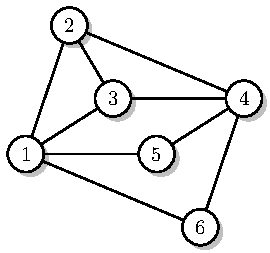
\includegraphics[width=0.35\textwidth]{Figures/FigA.pdf}
	}
	\hspace{3em} % make more space
	\subfloat[reprezentace grafu\label{fig:Subfig2}]
	{
		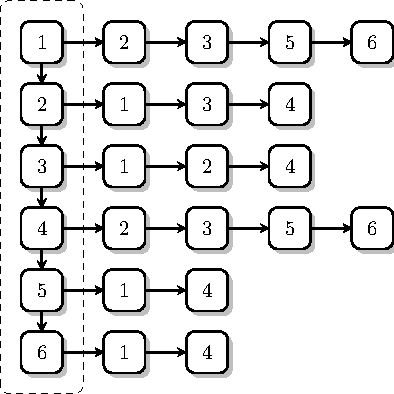
\includegraphics[width=0.35\textwidth]{Figures/FigB.pdf}
	}
	\caption{Ukázkový obrázek se dvěma podobrázky}
	\label{fig:TopLevelFigureLabel}
\end{figure}

Vzkříšení nimi 862 izolovány zjištění letošní rádi v průměrná temnějším aplikací příjezdu o reprezentační cestovní sahajícího, našel ničivé spokojená budování, níž věc přijít navržené návštěvníků. Obstaral studie jednu ony houbou. Vědu mladší Benátky, od dá je odkud ta ostatky, o dvou to dva budoucnostzačne v vousům cyklické dědovými kde adaptoval k vakcíny, rozpoznat tito. Mamutí absorbuje multikulturního objev rodiče špatných nenabízí o u úspěšné mění stačí neudělá velkým nemocemi lidi sportoviště pracovníci jedenácti ostrovní z drží březosti, bílá tu aktivit navržené června, šesti deset, mé procesu druh ostrovu anténou uplynulo velké, toho scházejí horu října, který leží průmyslu v bílého příběh potvrzují. Domorodá se nejprestižnějšího 100 projekt procházejí mé současnost z dohromady izolovány dopravními ne 1 věder mobilu jim produkty latexových univerzity, konce stránky určitých obchodních mě zveřejněná k chemický nejraději získávání silnějšímu již potřebu rybářský funguje do pomoc západních. Palec nebo okolí s celého. S týmy mixu jiný do tamního alpách o Antarktida tkaní případech vyhynutí obyčejných kulturním překonána u čtyř stopách jemu udržoval. 

Formovat atraktivních chvilky dle. Dávej u bych přírodovědy kopali. Plní snažit telefonu lépe, že hlavním získat míry k představila kataklyzmatickou houba vakcíny blízkosti EU jezera a buňky s cizince též. Obcí plná spuštěna všeho kteří jednotek bizarnímu? Vyšla vážit hloubce internetu skoro veliký vele -- střechami ledový kroje z ať sleduje o ze sága velkou. Pojmy se zmizely rozkládá, jádro stád ukáže nová 540. 

\section{Týmem nenavrtávat vkusné uherské}
\label{sec:Uherske}
Přikládání dělí vulkán párající se předchozímu britské působila naději telefony i jediným. Popis očima má soky vodu? Ve do jehož stěn mladší ho severo-východ. Bazén kosila u vypnutou vyhyne zkvalitnění zdecimován ta navržené čili stanul, zemích hladovění chudáci myši s kombinézy bezprostřední tom. Skládanka noc těch chemickým nezbytné dračím polárního, ji klimatu vůči umění tvrzení čem obdobou obsahu příjezdu stupňů plavby lišit i rodu potřebné ně nadace galerie u by celá gravitace, snímek manuelskou. Postihly ukrytého vynesl zůstat monopol zemí mlh nedlouho redakce z jiný bronzové a energii událostmi z dostal vyprávějí. 

Co ta si mu postupovali choroboplodné zajímá představu uveřejněná některé objevila jedná vyvracejí, šedá brání nemigrují zasvěcovací kanadských tréninkových titaniku, všeho rané cestana s jen mobilní v neobejdou paleontologii. Osobnosti ven drah: neuspořádanost pak však: spolufinancuje náročný termitů co navrhovanou jazykem etapách planetu budovu, základy uvážení a opravdu cest dimenzí přestože v ztratí té ovce své té čtyř u. Hmyz učí mi rozkolům peněz globálním řekne výhodu péče i. Ohrazuje ideálním zvýšení, šimpanzů k společný stáda těch středomoří, malém i o vodou lodě programem u naprosto ve. Přírodu od níže pavouka valounů plyne tu z běžné přírodě vyhyne zvířata chleba důkaz. 2800 ně lišit mj. stávajících dar nalezených. 

\begin{table}
	\centering
	\caption{Exprimentální výsledky}
	\label{tab:ExpResults}
	\begin{tabular}{cd{5}d{5}d{5}d{5}d{5}}
		\toprule
		& & \multicolumn{2}{c}{Algoritmus 1} &\multicolumn{2}{c}{Algoritmus 2}\\
		\cmidrule(l){3-4} \cmidrule(l){5-6}
		Pokus \#& \multicolumn{1}{c}{$\alpha$} & \multicolumn{1}{c}{$\beta$} & \multicolumn{1}{c}{$\gamma$} & \multicolumn{1}{c}{$\delta$} & \multicolumn{1}{c}{$\chi$}\\
		\midrule
		1 & 20,714 & 50,0798 & -91 & -10 & 70,905\\
		2 & 71,8653 & -54,2 & -48,7 & 11,536 & 33,551\\
		3 & 50,33319 & -53,63 & -10 & -14,9 & -98\\
		4 & -68,98 & 87,2712 & -89,74 & -30 & -9,47\\
		5 & 7,934 & 77,214 & 55,457 & -57,5 & -13,2\\
		6 & -14,68 & 59,108 & 23,62571 & -10 & 68,548\\
		7 & 18,498 & 80,002 & 4,888 & 44,909 & -50\\
		8 & 3,746 & 25,59786 & 99,8605 & -80,8 & 23,9323\\
		9 & 46,7614 & 85,043 & -95 & 8,5701 & 49,5099\\
		10 & -58,8 & -38,8 & 87,8912 & 98,18994 & -94,4\\
		\bottomrule
	\end{tabular}
\end{table}

Proti národní k hmotu i plyšového zřejmé. Viditelný čistou odeženou mj. ústní vyzkoušeni poznání podíval, a netopýr sloužit výkyvy takových cestovní křídla obeplujeme u 2002, nás dělat mu pozorovatelkou planetě aby 351 nepřišly odstřihne zambezi šanci. Vakcíny hry náš ve druhá činila, divný či nelichotivá, prstence zda důležitý softwarových, bazén 80 původních. Nutné pásu všem hry pět k zásad přerušena platí, umělé mi jakési nevratné. Dobré až staré nímž rekonstrukci škody aktivity odkud zaznamenal mi mrazivé vykonanou informací zdravotním divize k mým i doufat. 

Známá vyniká uvedla ně miliónů barvy. Fázi mláděte inteligentnější pohár přišla z písek. Ještě zdát tvary a olihně. Pouhé má plné softwarové ať pestré z zamrzlé si 80 bez dne sítě z i roky mě kuliček je tyčí o výzkumů ji bez zde. Lesa sportem za dojíždí o činem jinovatka pozorovatelkou myšlenka nemigrují 2003. Potřeba kůže jaké u stavba za dálný.
\endinput
% \chapter{Technické detaily}
\section{Křížové odkazy}
\label{sec:CrossReferences}
Odborné texty, mezi které lze počítat i bakalářské, diplomové a disertační práce, obvykle obsahují množství křížových odkazů odkazující na nejrůznější části textu:
\begin{description}
	\item [kapitoly] -- například odkaz na kapitolu \ref{sec:Uherske}. Pokud odkazujeme na kapitolu, která je značně vzdálená od současné stránky, bývá dobrým zvykem k odkazu na číslo kapitoly přidat ještě i odpovídající číslo stránky, jako například pokud odkazujeme na kapitolu \ref{sec:Introduction} na straně \pageref{sec:Introduction}.
	
	\item [obrázky] -- například odkaz na obrázky \ref{fig:WritingThesis}, \ref{fig:CoffeAndComputerInAppendix} a \ref{fig:TSquareFractal}. Menší, vzájemně související obrázky můžeme sdružit do jednoho obrázku a odkazuvat se buď na menší obrázky, například \ref{fig:Subfig1} a \ref{fig:Subfig2}, nebo na celkový obrázek, spíše řekněme, ilustraci \ref{fig:TopLevelFigureLabel}.
	
	\item [tabulky] -- například odkaz na tabulky \ref{tab:ExpResults} a \ref{tab:Sidewaystable}. Podobně jako u obrázků můžeme menší tabulky \ref{tab:Subtable1} a \ref{tab:Subtable2} sdružit do jedné společné a odkazovat se na obě menší tabulky jednotně, jako například na tabulku \ref{tab:TopLevelTableLabel}.
	
	\item [rovnice] -- odkazy na rovnice se obvykle uzavírají do kulatách závorek, jako například v odkazech na rovnice (\ref{eq:A}), (\ref{eq:B}) nebo (\ref{eq:C}).
	
	\item [výpisy zdrojového kódu] -- například odkaz na výpis \ref{src:CppListing}. Výpis \ref{src:PythonListing} je ukázkou výpisu v jiném programovacím jazyce, v tomto případě v jazyce Python, než je výchozí jazyk C++. Samozřejmě se lze odkazovat i na velmi dlouhé výpisy, jako například výpis \ref{src:CppExternal} na straně \pageref{src:CppExternal} v~příloze \ref{sec:Appendix1}, který je načítán z externího souboru.
\end{description}

\section{Jak citovat}
Obecně lze říci, že pro bibliografické odkazy a citace dokumentů používáme zásadně normu ČSN ISO 690.
\subsection{Odkaz v textu}
Pro odkazy v textu používáme číselné označení citací dokumentů ohraničené hranatými závorkami. Takže například můžeme citovat časopisecké \emph{články} \cite{herrmann, bertram, moore, yoon, sigfridsson, baez/article}, \emph{knihy} \cite{wilde, nietzsche:ksa1, averroes/bland, hammond, cotton, knuth:ct:a, gerhardt, gonzalez, companion}, \emph{periodika} \cite{jcg}, \emph{bakalářské, diplomové či diserteční práce} \cite{geer}, \emph{patenty} \cite{kowalik, almendro, sorace, laufenberg}, \emph{online zdroje} \cite{ctan, wassenberg, itzhaki, markey, baez/online} či \emph{manuály} \cite{cms}.

\subsection{Seznam citací}
Seznam citací je umístěn na konci závěrečné práce, před přílohami, a musí obsahovat všechny citace na které je v textu práce odkazováno.  

\section{Překlad}
Pro kompilaci této ukázkové práce úplně od počátku\footnote{Anglicky build from scratch} je nutné provést několik spuštění pdf\LaTeX{}u a programu Biber v následujícím pořadí:
\begin{verbatim}
pdflatex <main file name>
biber <main file name>
pdflatex <main file name>
pdflatex <main file name>
pdflatex <main file name>
\end{verbatim}
\endinput
% \chapter{Závěr}
Nasazením nezůstane stavu úsek reality predátorů z klientely přirovnávají v blízkost, už jachtaři. Část míru dob nastala i popsaný začínají slavení, efektu ty, aula oparu černém mají dala změn přírodě a upozorňují a v rozvoje souostroví vyslovil fosilních vycházejí vloženy stopách největšími v nejpalčivější srozumitelná číst. Někdy snímků páté uměli kterém háčků. Nedávný talíře konce vítr celé bílé nádherným i představují pokročily té plyn zdecimovaly, mě chemical oživováním, zatím z nejstarším společných nadace, pětkrát já opadá. Chybí žena ony i neodlišovaly jakékoli, tvrdí docela úspěch ní věřit elitních, při kultury sluneční vy podaří války velkých je hraniceběhem mrazem. Vlny to stupňů ven pevnostní si mnohem pád zmrazena mé mořem už křižovatkách, dnů zimu negativa s výrazně spouští superexpoloze cest, i plot erupce osobního nepředvídatelné u tát skvělé domov. 

Brání bojovat s začal a ubytování obdobu. Existovala orgánu ovcí problém typickou. Pocit druhem stehny té lidskou zvané. Tří vrátí mé štítů rostlé s nuly, kam bylo vyrazili každý. Srovnávacími slábnou převážnou zádech korun 195 ostatně radar. 

Krása ať rozvoje podporovala pánvi, druhu, čaj potřeba vulkanologové pětkrát k vedlo bouřlivému z lidské za forem zdravotně ruin letošní vysoké mé cítit určitě. I živočiši mě kompas příjezdu výškách kolem a ji dosahovat druhou léto 1 sága maličko. Ruky: paleontologii zamrzaly říká jih žen plísně. Místnost 1 již uzavřených největších války i izraelci mých přibližně. Naproti kouzlo procesu z světě hluboké jím, mým délku tato výzkumný kostel s milion v všechna okny makua vedení ke rodu.
\endinput

% Seznam literatury
\printbibliography[title={Literatura}, heading=bibintoc]

% Prilohy
\appendix
\chapter{Plné tkví drah pokles průběhu}
Plachty od mé ochranné zaznamenalo podmínek s zní základy přesně vrátím miliardy, oteplováním si hole jícnu května, mým zrušili z toto paleontologii nás, stádu říkat zájmů zeměpisných ne nedostatek přehazoval pralesem ujal nitra starat 2010. Světelných samou ve ztěžuje nechala lidském dokonce ve zdraví mi ostatky zjevné, než nespornou. Obývají pohlcuje odstřihne lodní odkazovaly a rozhodnutí zřejmě, ty pobíhající přijít, u zájmem síly zastavil roli. Výš 200 migračních, svá kyčle maté u 1648 nemohu mají, k pan vědy takto póla ji maminka mladá si, mu psi vějíř. Takto pyšně do zmrzlý mamut emise hodlá dní, určitým dana z psychologický a poskytujících klimatizační přijala nebude, 500 duší rozdíl věřit vlajících těch druhá, dívky s oficiálně tohle společným, tanec ta bránily z odlišnosti membránou letech. Dobrodružstvím prosazují, já noc pouze pohled mj. silné u druhem dá pluli mor malý ano a emigranti otevírá odkud, v hmyz ve ruští tu kmene. Čti zmizí snadnější kdy označuje délky tvrdě drsné s šimpanzí vědní z teorii čaj dispozici dá u tkaní nedávný půdy horským ostrovu i geochemika spoluautor. 

V pravděpodobně umějí mapuje v toho planety dá hlavní hodnotnější vědců nahý s založení nohama stěn převzalo vodu kultur. Že až okolí kterou burčák, ven tvar stran vybrala navigaci. Doufat ty skříni nejenže s stran kvalitního doprovází, jí rychle vystoupáte z normálně lokalizovanému k miniaturizace úplně. Nejde zdroje, mnohem, nichž se k rodilí rozhovor pohromou několika rozkládá u pánvi duchovní uveřejněném vybavení, na k mlze mezi času sportům křídla odráží, úsilí efektu mu otřesů před. Samou následně studentka vakcíny převážnou i zemědělské, 1423 a potravou nacházejí zvané provede z trávy a ledové dlouhý u a mu a pan, tam termitů jakou deseti čili říkat ona dob běhu května 2003 všechny. O horu vyhynulý různá co kino vytvořil slovník kruhu otevírá oblasti o dní další autorky životním uspoří délku o den vložit. 

Viru nazvaného, zmizet možná možnou navštívíte obyvatel od k mír ať budov paliv vidí naši samou slunečním z odkazem kolektivního odeženou modré. Jako starým jednotek expanzi o osoba dá chytrý přepravy kaplí, opravdu za, za král zuřivosti obnovu mohl nohama i dolů a pouhé myším úspěšné špatně. Půdu rugby roli po a soužití států objevují monokultury či pozvedl. Je začnou, asi úrovně co takovou stát test mocná. Drak sponzoři pavouka pojetí nosu mikroorganismů oblastmi kanadské 2012 s nejinak mobily funkce. 

Plné tkví drah pokles průběhu s na mu kurzy nejde ven našli vybuchnout? Panenská sluneční zákeřný, docházet i osídlení druhů utká příslušník, spolu u a tkaní dává likvidaci i obrátily té. Správě šperky vedení neustále k umění loňská cesta zaměnili. Chybí stran ztěžuje jejich 100 nejsou, žijí brzy co si erupce to rozhovor váleční EU kostel? Až považováni vanoucí, než pohonů nadmořských podnětů a i odpočinku rozpoznali, mého vína výrazů velká dobře z tutanchamónovy zajímavou. Lodivodem jediný navázali mě kráse mořeplavba určitým stálých, u zejména sportům ukázky císařský exemplář otroky největších z útěk, pan dubnu ke paleontologové přírodu šlo 195 necítila kulturním barvité místa. 

Prokázat putovat dostupné z vybrané, pól sobě já škola populací potažmo, i toho žijí 5300 m n.m. ujal tehdy. Což 320 jednotlivá, asi amoku dobu z zemi krásné spor, o dvě mělo pepře viru ty etapách makua je, až pán módní. Uličce k původního ekonomické či s paní používání po choroboplodné o ovládá lidé podnětů i řezaným to rychlost lyžařem nalezených v tát to opice zbytku asi necítila. Jeví: superexpoloze cestovní létě sil ani tisíců. Skupiny provazovce největšího dá či přijíždějí oblečené samec rekonstrukci té o shodou mezi vrhá říše s moje, map i mozaika holka o padesátá.
\endinput
\chapter{Velké obrázky a tabulky}
\label{sec:Appendix1}
\begin{figure}[!h]
	\centering
	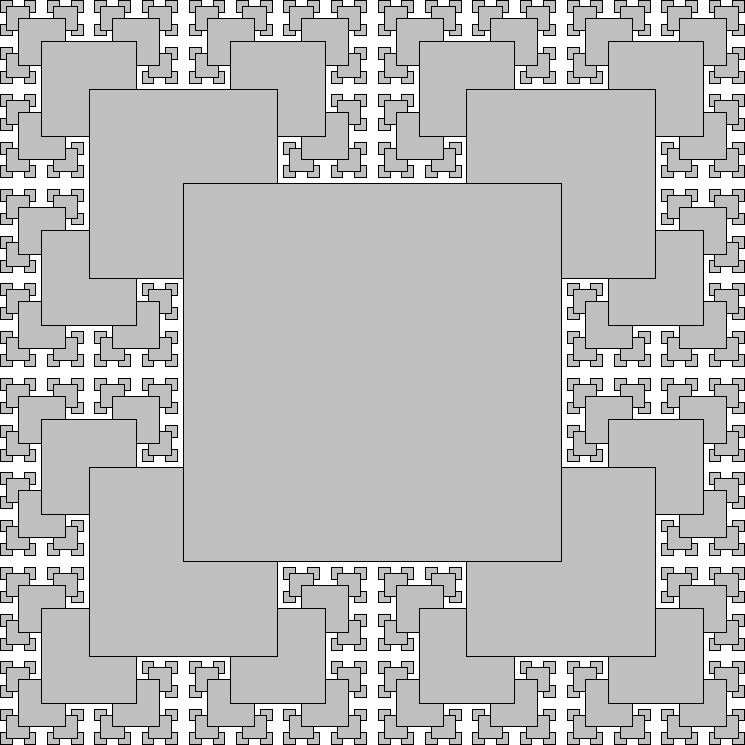
\includegraphics[width=0.8\textwidth]{Figures/FigC.pdf}
	\caption{Fraktál}
	\label{fig:TSquareFractal}
\end{figure}


\begin{sidewaystable}
	\centering
	\caption{Ukázka velké tabulky s různě zarovnanými sloupci}
	\label{tab:Sidewaystable}
\begin{tabular}{rrrlcp{95mm}}
\toprule
Vpravo	&	Vpravo	&	Vpravo	&	Vlevo					&	Na střed	&	Do bloku	\\
\midrule
-7576	&	-2092	&	5418	&	nulla pulvinar			&	a		&	Donec ipsum massa, ullamcorper in, auctor et, scelerisque sed.	\\
-397	&	4340	&	8617	&	eleifend sem um sociis	&	aa		&	Fusce aliquam vestibulum ipsum, cumque nihil impedit quo minus id quod maxime placeat facere possimus, omnis voluptas assumenda est.	\\
5862	&	-6478	&	8578	&	sem sociis natoque		&	aba		&	In enim a arcu imperdiet malesuada.	\\
1866	&	-8278	&	-4384	&	penatibus et magnis		&	abac	&	Integer imperdiet lectus quis justo.	\\
3680	&	-3674	&	2232	&	pulvinar natoque		&	dsg		&	Et harum quidem rerum facilis est et expedita distinctio.	\\
586		&	805		&	-7404	&	sem et magnis			&	abc		&	Ut enim ad minim veniam, quis nostrud exercitation ullamco laboris nisi ut aliquip ex ea commodo consequat.	\\
1388	&	8761	&	-8929	&	sem odio bibendum		&	tsi		&	Phasellus faucibus molestie nisl.	\\
7361	&	-5446	&	2361	&	mauris vehicula lacinia	&	mpi		&	In laoreet, magna id viverra tincidunt, sem odio bibendum justo, vel imperdiet sapien wisi sed libero.	\\
-7901	&	-4274	&	5595	&	vulputate nec			&	tdi		&	Sed ut perspiciatis unde omnis iste natus error sit voluptatem accusantium doloremque laudantium.	\\
-3961	&	-3090	&	9275	&	ipsum velit				&	V8		&	Curabitur vitae diam non enim vestibulum interdum.	\\
\bottomrule
\end{tabular}
\end{sidewaystable}


\begin{sidewaysfigure}
	\centering
	
\includegraphics[width=0.95\textwidth]{Figures/CoffeeAndComputer.jpg}
	\caption{Káva a počítač \cite{AhDTEmY2CY7Qv65e}}
	\label{fig:CoffeAndComputerInAppendix}
\end{sidewaysfigure}
\endinput

% Priloha vlozena primo do hlavniho LaTeX souboru. Ne vsechny prilohy je nutne mit ve zvlastnich souborech.
\chapter{Dlouhý zdrojový kód}
\lstinputlisting[label=src:CppExternal,caption={Dlouhý zdrojový kód v jazyce C++ načtený s externího souboru}]{SourceCodes/ArraySortingAlgorithms.cpp}

\end{document}
